
%\section*{Thesis overview}

	\newcommand{\relevance}{\underline{\textbf{\relevanceTXT}}}
%	\newcommand{\progress}{\underline{\textbf{\progressTXT}}}
	\newcommand{\goal}{\underline{\textbf{\goalTXT}}}
	\newcommand{\scientifictasks}{\underline{\textbf{\scientifictasksTXT}}}
	\newcommand{\scientificnovelty}{\underline{\textbf{\scientificnoveltyTXT}}}
	\newcommand{\importance}{\underline{\textbf{\importanceTXT}}}
%	\newcommand{\methods}{\underline{\textbf{\methodsTXT}}}
	\newcommand{\statements}{\underline{\textbf{\statementsTXT}}}
	\newcommand{\validity}{\underline{\textbf{\validityTXT}}}
	\newcommand{\approbation}{\underline{\textbf{\approbationTXT}}}
	\newcommand{\implementation}{\underline{\textbf{\implementationTXT}}}
%	\newcommand{\contribution}{\underline{\textbf{\contributionTXT}}}
	\newcommand{\refs}{\underline{\textbf{\refsTXT}}}
\chapter*{Synopsis}
\addcontentsline{toc}{chapter}{Synopsis} 
\section*{Thesis overview}

%	\section*{The goal}
%	\section*{Scientific tasks:}
%	\section*{Scientific novelty}
%	\section*{Scientific statements:}
%	\section*{Practical importance}
%	\section*{Reliability and the validity}
%	\section*{Implementation of the obtained results}
%	\section*{Approbation}
%	\section*{Publication}
%	\section*{Author contribution}
%	\section*{The structure}
%	\section*{MAIN CONTENTS OF WORK}


  {\relevance} 
  Quantum informatics is a field of knowledge that combines elements of the photonics and the theory of information. Quantum bits, or qubits, are used as the basic units of quantum information science. Qubit is a system that can be in a superposition state and used to store, calculate and transmit information. One of the promising areas of quantum informatics are a quantum calculations and a quantum memory -- the main components of a quantum computer -- a totally new type of computing device that works on the fundamental principles of quantum mechanics. The transmission of a quantum state at various distances, or quantum teleportation, is another promising application of quantum informatics. The generation of a symmetric bit sequence by the quantum methods, or quantum key distribution (QKD), was formed as a scientific direction in the 80's of the 20th century. This direction is advanced in terms of application. In quantum communication systems (QCS), through the use of quantum states, two or more legitimate users can distribute symmetric bit sequences, which can subsequently be used as keys for encoding information, so that any eavesdropping attempts of the communication channel will be detected by the increased error rate.
  
Differences between physical implementations of QCS from ideal models used in theoretical approaches can be the basis for conducting various types of attacks on equipment used in this systems. It was previously shown that gated single-photon detectors (SPD) of several commercially available QKD systems were vulnerable to attack by the eavesdropper. It is noteworthy that exposure can be carried out even by optical methods. Eavesdropping can be made directly from a quantum channel that connects legitimate users. In practice, optical fiber is most often used as a medium for the transferring of quantum states. Single photons and their properties are usually used for that purposes.
	
This type of attack is called a <<faked-states attack>> (FSA). It is based on the fact that for the detection of photons, a detector based on avalanche photodiodes (APDs) operating in the Geiger mode, or photon counting mode, is used. With this approach, in the absence of additional protective measures, the attacker has the ability to use the powerful constant optical radiation to carry the detector out from the Geiger mode to the linear mode (so-called <<blinding>>) and provoke triggering due to the use of powerful short pulses. Thus, the feasibility of complete control of the single-photon registration node, became critical for QKD protocols, and as a result, leads the eavesdropper to imperceptible obtaining of the full key correlating with that of legitimate users.
	

There are several ways to counter this type of attack, but in practice most of them have not been tested in quantum hacking laboratories. Several countermeasures that were analyzed and investigated have included counterattacks and hacking methods that were not taken into account by the developers of countermeasures.
	
The most effective countermeasure against the well-known types of attacks on detector side is the implementation of a  quite new QKD architecture that is resistant to attacks on measuring equipment (Measurement-Device-Independent, or MDI). With this approach, it is initially assumed that the single-photon registration unit is moved outside the sender and receiver blocks and is completely accessible to the eavesdropper. However, such an approach is characterized by a higher level of complexity of implementing the optical scheme and lower characteristics with respect to QKD systems with a point-to-point topology with a registration node in one of the blocks.
	
One of the promising approaches is the method of quantum communication at subcarrier-wave quantum key distribution (SCW~QKD). Its distinctive feature is the carrying of the quantum channel out to the sidebands generated as a result of modulation. This ensures high resistance to external factors and spectral efficiency, as well as good performance in the ratio of the key formation speed to the distance between the sender and receiver units. However, as part of this type of system for small and medium distances (up to 100~km), single-photon detectors based on the APD are also used, and the resistance to attacks on the measuring equipment of SCW~QKD systems has not been investigated.
	
	
% Обзор, введение в тему, обозначение места данной работы в
% мировых исследованиях и~т.\:п., можно использовать ссылки на~другие
% работы\ifnumequal{\value{bibliosel}}{1}{~\autocite{Gosele1999161}}{}
% (если их~нет, то~в~автореферате
% автоматически пропадёт раздел <<Список литературы>>). Внимание! Ссылки
% на~другие работы в разделе общей характеристики работы можно
% использовать только при использовании \verb!biblatex! (из-за технических
% ограничений \verb!bibtex8!. Это связано с тем, что одна
% и~та~же~характеристика используются и~в~тексте диссертации, и в
% автореферате. В~последнем, согласно ГОСТ, должен присутствовать список
% работ автора по~теме диссертации, а~\verb!bibtex8! не~умеет выводить в одном
% файле два списка литературы).
% При использовании \verb!biblatex! возможно использование исключительно
% в~автореферате подстрочных ссылок
% для других работ командой \verb!\autocite!, а~также цитирование
% собственных работ командой \verb!\cite!. Для этого в~файле
% \verb!Synopsis/setup.tex! необходимо присвоить положительное значение
% счётчику \verb!\setcounter{usefootcite}{1}!.
% 
% Для генерации содержимого титульного листа автореферата, диссертации
% и~презентации используются данные из файла \verb!common/data.tex!. Если,
% например, вы меняете название диссертации, то оно автоматически
% появится в~итоговых файлах после очередного запуска \LaTeX. Согласно
% ГОСТ 7.0.11-2011 <<5.1.1 Титульный лист является первой страницей
% диссертации, служит источником информации, необходимой для обработки и
% поиска документа>>. Наличие логотипа организации на~титульном листе
% упрощает обработку и~поиск, для этого разметите логотип вашей
% организации в папке images в~формате PDF (лучше найти его в векторном
% варианте, чтобы он хорошо смотрелся при печати) под именем
% \verb!logo.pdf!. Настроить размер изображения с логотипом можно
% в~соответствующих местах файлов \verb!title.tex!  отдельно для
% диссертации и автореферата. Если вам логотип не~нужен, то просто
% удалите файл с~логотипом.

% \ifsynopsis
% Этот абзац появляется только в~автореферате.
% Для формирования блоков, которые будут обрабатываться только в~автореферате,
% заведена проверка условия \verb!\!\verb!ifsynopsis!.
% Значение условия задаётся в~основном файле документа (\verb!synopsis.tex! для
% автореферата).
% \else
% Этот абзац появляется только в~диссертации.    ----- условие выполняется как else в обоих случаях (для диссертации и реферата)
% Через проверку условия \verb!\!\verb!ifsynopsis!, задаваемого в~основном файле
% документа (\verb!dissertation.tex! для диссертации), можно сделать новую
% команду, обеспечивающую появление цитаты в~диссертации, но~не~в~автореферате.
% \fi

% {\progress}
% Этот раздел должен быть отдельным структурным элементом по
% ГОСТ, но он, как правило, включается в описание актуальности
% темы. Нужен он отдельным структурынм элемементом или нет ---
% смотрите другие диссертации вашего совета, скорее всего не нужен.

{\goal} of this dissertation is to investigate a feasibility of the secret key eavesdropping by detector side channel attacks of SCW~QKD systems and to develop countermeasure methods.


{\scientifictasks}:
\begin{enumerate}
  \item Investigate vulnerability to blinding of the SPD used in SCW~QKD.  

  \item Estimate the eavesdropper limits in case of successfully controlling detector side. 

  \item Develop an optical scheme for monitoring possible eavesdropping.

  \item Investigate a measurement-device independent QKD protocol based on multi-mode weak coherent states used in SCW~QKD. 
\end{enumerate}


{\scientificnovelty} is specified by the following new results:
\begin{enumerate}
  \item It is experimentally demonstrated the vulnerability of SCW~QKD to faked-state attacks.
  \item For the first time it is shown that the SCW~QKD basic optical scheme provides an advantage and could be updated for monitoring the bright light.
  \item It is proposed and experimentally studied the feasibility of twin-field quantum key distribution based on multi-mode coherent phase-coded states. The detection node is moved away to untrusted relay. The nontrivial interference is obtained. Key rate estimation shows that SCW approach can beat well-known fundamental limits of repeaterless quantum communications (linear bound).
\end{enumerate}

{\statements}
\begin{enumerate}

  \item Single-photon detector based on avalanche photodiode with 100~MHz external gating could be moved out from photon-counting mode by bright light illumination no less than 35 nW. It could be triggered by optical pulses with energy more than 15,4 fJ regardless of their repetition rate.
  \item The frequency conversion of the control signal by phase modulation on the radio frequency mode allows to detect a faked-state attack by monitoring a carrier's frequency.
  \item The use of weak coherent multi-mode states with phase coding makes it possible to implement a protocol that is resistant to control by an illegitimate user of measuring device.
  \item In result of interference of quantum states at sidebands on a symmetrical beam splitter placed in untrusted detection node, the spectral separation of the quantum signal and the signal at the central wavelength occurs with their independent registration in different beamsplitter outputs. 
  %  \item Double distance increasing is performed by using twin-field approach for multi-mode weak coherent phase-coded states. 
  %  \item Показана возможность двукратного увеличения дальности квантовой рассылки ключа на боковых частотах посредством применения недоверенной системы регистрации квантовых состояний. 
 
\end{enumerate}
{\influence} 

Разработанные методы и подход позволили однозначно определить уязвимость коммерчески доступных детекторов компании id Quantique модели id210 к выведению из режима Гейгера оптическими средствами. В связи с чем доказана необходимость применения дополнительных мер защиты от атак на измерительный узел. Предложена схема, позволяющая производить активный мониторинг попыток <<ослепить>> детектор, благодаря использованию особенностей систем квантовой коммуникации на боковых частотах. Результаты внедрены в производство ООО "Кванттелеком". 

%  {\methods} \todo{TO DO} \ldots

%%%%%	{\defpositions}
%%%%%	\begin{enumerate}
%%%%%  \item Использование коммерческих детекторов одиночных фотонов на основе лавинных фотодиодов в режиме Гейгера модели id210 с частотой стробирования 100 МГц  требует применения дополнительных средств защиты от атаки с выведением из режима Гейгера при помощи коротких оптических импульсов с энергией не менее 15,4 фДж и при постоянном уровне оптической засветки средним уровнем мощности излучения не менее 35 нВт.  
%%%%%  \item Измерение величины оптического излучения на несущей частоте, отраженного от оптического фильтра, при помощи мониторного фотодиода в приемном блоке системы квантовой коммуникации на боковых частотах в диапазоне от 7 нВт до 2,93 мкВт с применением дополнительных мер в виде пассивного оптического аттенюатора номиналом 10 дБ для его защиты позволяет противостоять атаке с выведением детектора одиночных фотонов из режима Гейгера и навязыванием ключа нелегитимным пользователем. 
%%%%%  \item Метод квантовой коммуникации на боковых частотах позволяет реализовывать протокол, устойчивый к контролю нелегитимным пользователем измерительного оборудования. 
%%%%%  \item В результате интерференции квантового фазомодулированного сигнала на боковых частотах на симметричном светоделителе в схеме квантовой рассылки ключа с узлом регистрации, независящим от легитимного пользователя, происходит спектральное разделение квантового сигнала и сигнала на центральной длине волны с их независимой регистрацией в разных плечах светоделителя. 
%%%%%%%  \item Показана возможность двукратного увеличения дальности квантовой рассылки ключа на боковых частотах посредством применения недоверенной системы регистрации квантовых состояний. 
%%%%%%%%\end{enumerate}
% В папке Documents можно ознакомиться в решением совета из Томского ГУ
% в~файле \verb+Def_positions.pdf+, где обоснованно даются рекомендации
% по~формулировкам защищаемых положений.




{\reliability} полученных результатов обеспечивается применением утверждённых методик проведений экспериментальных исследований и аттестованного оборудование. Математическое моделирование и обработка данных, полученных в результате экспериментов, осуществлялось с использованием пакетов прикладных программ MathCad и Excel. Результаты находятся в соответствии с результатами, полученными другими авторами.


{\probation}
Основные результаты работы докладывались~на:
%перечисление основных конференций, симпозиумов и~т.\:п. 
\begin{enumerate}
	\item ICQOQI 2019, Минск, Беларусь, 13 - 17 мая 2019
	\item XLVIII научная и учебно-методическая конференция Университета~ИТМО, Санкт-Петербург, Россия, 29 января - 1 февраля 2019
	\item QCrypt 2018, Шанхай, Китай, 27 - 31 августа 2018
	\item 18th International Conference on Laser Optics ICLO 2018, Санкт-Петербург, Россия, 4 - 8 июня 2018
	\item VII Всероссийский конгресс молодых ученых, Санкт-Петербург, Россия, 17 - 20 апреля 2018
	\item XLVII научная и учебно-методическая конференция Университета ИТМО, Санкт-Петербург, Россия, 30 января - 2 февраля 2018
\end{enumerate}

% {\contribution} Автор принимал активное участие \todo{TO DO} \ldots

%\publications\ Основные результаты по теме диссертации изложены в ХХ печатных изданиях~\cite{Sokolov,Gaidaenko,Lermontov,Management},
%Х из которых изданы в журналах, рекомендованных ВАК~\cite{Sokolov,Gaidaenko},
%ХХ --- в тезисах докладов~\cite{Lermontov,Management}.

\ifnumequal{\value{bibliosel}}{0}{% Встроенная реализация с загрузкой файла через движок bibtex8
    \publications\ Основные результаты по теме диссертации изложены в XX печатных изданиях,
    X из которых изданы в журналах, рекомендованных ВАК,
    X "--- в тезисах докладов.%
}{% Реализация пакетом biblatex через движок biber
%Сделана отдельная секция, чтобы не отображались в списке цитированных материалов
    \begin{refsection}[vak,wos,scopus,papers,conf]% Подсчет и нумерация авторских работ. Засчитываются только те, которые были прописаны внутри \nocite{}.
        %Чтобы сменить порядок разделов в сгрупированном списке литературы необходимо перетасовать следующие три строчки, а также команды в разделе \newcommand*{\insertbiblioauthorgrouped} в файле biblio/biblatex.tex
        \printbibliography[heading=countauthorvak, env=countauthorvak, keyword=biblioauthorvak, section=1]%
        \printbibliography[heading=countauthorwos,env=countauthorwos, keyword=biblioauthorwos, section=1]%
        \printbibliography[heading=countauthorscopus,env=countauthorscopus, keyword=biblioauthorscopus, section=1]%
	\printbibliography[heading=countauthorconf, env=countauthorconf, keyword=biblioauthorconf, section=1]%
        \printbibliography[heading=countauthorothers, env=countauthorothers, keyword=biblioauthorothers, section=1]%
        \printbibliography[heading=countauthor, env=countauthor, keyword=biblioauthor, section=1]%
        \nocite{%Порядок перечисления в этом блоке определяет порядок вывода в списке публикаций автора
                JOT,Chistyakov_2016,%
		Chistiakov:19,%
		scbib1,%
                confbib1,confbib2,%
                bib1,bib2,%
        }%
	\publications\ Основные результаты по теме диссертации изложены в 13 печатных изданиях. 10 из которых изданы в журналах, рекомендованных ВАК, 3 в тезисах докладов. 
	
	\section*{Работы автора по теме диссертации}
{Статьи в журналах, рекомендованных ВАК: }
\begin{enumerate}\addtolength{\itemsep}{-0.5\baselineskip}
\renewcommand{\labelenumi}{[\theenumi]}
\item Vladimir Chistiakov, Anqi Huang, Vladimir Egorov, and Vadim Makarov, Controlling single-photon detector ID210 with bright light, Opt. Express 27, 32253-32262 (2019)
\\
\item Чистяков В.В., Гайдаш А.А., Козубов А.В., Глейм А.В. Исследование интерференции слабых когерентных многомодовых состояний для задач квантовой коммуникации с недоверенным приемным узлом // Научно-технический вестник информационных технологий, механики и оптики. 2019. Т. 19. № 6. doi: 10.17586/2226-1494-2019-19-6
\\
\item    Gleim A.V., Egorov V.I., Nazarov Y.V., Smirnov S.V., Chistyakov V.V., Bannik O.I., Anisimov A.A., Kynev S.M., Ivanova A.E., Collins R.J., Kozlov S.A., Buller G. Secure polarization-independent subcarrier quantum key distribution in optical fiber channel using BB84 protocol with a strong reference//Optics express, IET - 2016, Vol. 24, No. 3, pp. 2619-2633
\\
\item  Глейм А.В., Егоров В.И., Чистяков В.В., Смирнов С.В., Банник О.И., Булдаков Н.В., Гайдаш А.А., Козубов А.В., Васильев А.Б., Кынев С.М., Хоружников С.Э., Козлов С.А., Васильев В.Н. Квантовая коммуникация на боковых частотах со скоростью 1 Мбит/с в городской сети // Оптический журнал -2017. - Т. 84. - № 6. - С. 3-9
\\
\item  Chistyakov V.V., Kynev S.M, Smirnov S.V., Nazarov Y.V., Gleim A.V. Achieving high visibility in subcarrier wave quantum key distribution system // Journal of Physics: Conference Series, IET - 2016, Vol. 735, No. 1, pp. 012085
\\
\item V. V. Chistyakov, A. V. Gleim, V. I. Egorov, Yu. V. Nazarov. Implementation of multiplexing in a subcarrier-wave quantum cryptography system // Journal of Physics: Conference Series - 2014  vol. 541,  pp. 012078
\\
\item   Kynev S.M., Chistyakov V.V., Smirnov S.V., Volkova K.P., Egorov V.I., Gleim A.V. Free-space subcarrier wave quantum communication // Journal of Physics: Conference Series - 2017, Vol. 917, No. 5, pp. 052003
\\

\item    Gleim A.V., Nazarov Y.V., Egorov V.I., Smirnov S.V., Bannik O.I., Chistyakov V.V., Kynev S.M., Anisimov A.A., Kozlov S.A., Vasil'ev V.N. Subcarrier Wave Quantum Key Distribution in Telecommunication Network with Bitrate 800 kbit/s//EPJ Web of Conferences, IET - 2015, Vol. 103, pp. 10005
\\
\item    Gleim A.V., Egorov V.I., Nazarov Y.V., Smirnov S.V., Chistyakov V.V., Bannik O.I., Anisimov A.A., Kynev S.M., Collins R.J., Kozlov S.A., Buller G.S. Polarization insensitive 100 MHz clock subcarrier quantum key distribution over a 45 dB loss optical fiber channel // Conference on Lasers and Electro-Optics, CLEO 2015, IET - 2015, pp. 7182997
\\
\item Gaidash A.A., Kozubov A.V., Chistyakov V.V., Miroshnichenko G.P., Egorov V.I., Gleim A.V. Security conditions for sub-carrier wave quantum key distribution protocol in errorless channel // Journal of Physics: Conference Series - 2017, Vol. 917, No. 6, pp. 062014
\\
%\item  Gleim A.V., Chistyakov V.V., Bannik O.I., Egorov V.I., Buldakov N.V., Vasilev A.B., Gaidash A.A., Kozubov A.V., Smirnov S.V., Kynev S.M., Khoruzhnikov S.E., Kozlov S.A., Vasil'ev V.N. Sideband quantum communication at 1 Mbit/s on a metropolitan area network // Journal of Optical Technology - 2017, Vol. 84, No. 6, pp. 362-36
\\

\end{enumerate}
\noindent{ Другие публикации: }
\begin{enumerate}\addtolength{\itemsep}{-0.5\baselineskip}
\renewcommand{\labelenumi}{[\theenumi]}
\setcounter{enumi}{9}
\item   Чистяков В.В., Кынев С.М., Смирнов С.В., Назаров Ю.В., Глейм А.В. Обеспечение высокой видности в системе квантовой криптографии на боковых частотах // Сборник трудов IX международной конференции молодых ученых и специалистов «Оптика – 2015», с. 658-660
\\
\item Глейм А.В., Назаров Ю.В., Егоров В.И., Чистяков В.В, Смирнов С.В., Банник О.И., Кынев С.М., Иванова А.Е., Дубровская В.Д., Тарасов М.Г., Булдаков Н.В., Кузьмина Т.Б., Чивилихин С.А., Анисимов А.А., Рощупкин С.В., Рогачёв К.С., Хоружников С.Э., Козлов С.А., Васильев В.Н. Создание квантовой сети университета ИТМО //Сборник трудов VIII международной конференции «Фундаментальные проблемы оптики – 2014». Санкт-Петербург, 20-24 октября ,2014, С.3-4,  541 с. 
\\
\item А.В. Глейм, В.И.Егоров, А.А. Анисимов, Ю.В. Назаров, С.М. Кынев, А.В. Рупасов, В.В. Чистяков, А.А.Гайдаш, М.А. Смирнов, С.А. Чивилихин, С.А. Козлов Квантовая рассылка криптографического ключа по оптическому волокну телекоммуникационного стандарта на расстояние 200 км со скоростью 0.18 кбит/с // Cборник трудов III Всероссийская конференция по фотонике и информационной оптике Москва, НИЯУ МИФИ, 2014 с. 17-19
\\


\end{enumerate}

	
%	\setcounter{citeauthorscwostot}{\value{citeauthorscopus}} % вместе setcounter и addtocounter добавляют пробел между словами. По-этому они так раскиданы.
%        в~\arabic{citeauthor}~печатных изданиях,
%	\addtocounter{citeauthorscwostot}{\value{citeauthorwos}}
%	\arabic{citeauthorvak} из которых изданы в журналах, рекомендованных ВАК\sloppy
%	\ifnum \value{citeauthorscwostot}>0
%	, \arabic{citeauthorscwostot} "--- в~периодических научных журналах, индексируемых Web of Science и Scopus\sloppy
%	\fi
%	\ifnum \value{citeauthorconf}>0
%	, \arabic{citeauthorconf} "--- в~тезисах докладов.
%	\else
%	.
%	\fi
%    \end{refsection}
%    \begin{refsection}[vak,wos,scopus,papers,conf]%Блок, позволяющий отобрать из всех работ автора наиболее значимые, и только их вывести в автореферате, но считать в блоке выше общее число работ
%        \printbibliography[heading=countauthorvak, env=countauthorvak, keyword=biblioauthorvak, section=2]%
%        \printbibliography[heading=countauthorwos, env=countauthorwos, keyword=biblioauthorwos, section=2]%
 %       \printbibliography[heading=countauthorscopus, env=countauthorscopus, keyword=biblioauthorscopus, section=2]%
  %      \printbibliography[heading=countauthorothers, env=countauthorothers, keyword=biblioauthorothers, section=2]%
  %      \printbibliography[heading=countauthorconf, env=countauthorconf, keyword=biblioauthorconf, section=2]%
   %     \printbibliography[heading=countauthor, env=countauthor, keyword=biblioauthor, section=2]%
        
    %    \nocite{Chistyakov_2016}%vak
    %    \nocite{Gleim:15}
    %    \nocite{Gleim:16}
    %    \nocite{Gleĭm:17}
        
     %   \nocite{bib1}%other
     %   \nocite{confbib1}%conf
   \end{refsection}
}
% При использовании пакета \verb!biblatex! для автоматического подсчёта
% количества публикаций автора по теме диссертации, необходимо
% их~здесь перечислить с использованием команды \verb!\nocite!.
 % Характеристика работы по структуре во введении и в автореферате не отличается (ГОСТ Р 7.0.11, пункты 5.3.1 и 9.2.1), потому её загружаем из одного и того же внешнего файла, предварительно задав форму выделения некоторым параметрам

%Диссертационная работа была выполнена при поддержке грантов ...

%\underline{\textbf{Объем и структура работы.}} Диссертация состоит из~введения,
%четырех глав, заключения и~приложения. Полный объем диссертации
%\textbf{ХХХ}~страниц текста с~\textbf{ХХ}~рисунками и~5~таблицами. Список
%литературы содержит \textbf{ХХX}~наименование.

 \section*{Main contents of work}
 The \underline{\textbf{introduction}} substantiate the relevance of research carried out as part of this dissertation is substantiated, the goal is formulated, the tasks are set, the scientific novelty and practical significance of the work presented are stated.

 In \underline{\textbf{the first chapter}} with a review character, the main currently known methods for detecting single photons for use in quantum communication systems are considered. The analysis and comparison of various types of photon detectors are carried out, the choice of the single photon detector (SPD) studied in the work based on avalanche breakdown is justified. Possible attacks by a potential attacker on measuring equipment are shown, as well as known countermeasures against this type of attack.

%  картинку можно добавить так:
% \begin{figure}[ht]
%   \centering
%   
\includegraphics [scale=0.27] {latex}
%   \caption{Подпись к картинке.}
 %  \label{fig:latex}
% \end{figure}

% Формулы в строку без номера добавляются так:
% \[
%   \lambda_{T_s} = K_x\frac{d{x}}{d{T_s}}, \qquad
%   \lambda_{q_s} = K_x\frac{d{x}}{d{q_s}},
% \]

 \underline{\textbf{The second chapter}} is devoted to the study of a detector based on avalanche breakdown in a photodiode, which is used as measuring device for registering the result of interference of quantum states in a subcarrier-wave QKD system. This type of SPD is usually used for mid range distances of up to 100 ~ km with losses in communication lines less than 15~dB.

It's main advantages are following:
\begin{enumerate}
	\item High frequency trigger pulses - up to 100~MHz.
	\item The ability to supply strobe pulses from an external device (External gating mode).
	\item Wide range of setting the width of the operation window (gate) - from 0.5~ns to 25~ns.
	\item Setting the delay of opening the response window relative to the gate pulse (Trigger delay) in the range up to 10~ns with high resolution in time - 10~ps.
	\item Ability to set <<dead time>> in a wide range - from 0.1~μs to 100~μs.
	\item The ability to adjust quantum efficiency in increments of 2.5~\% in the range from 5~\% to 25~\%.
	\item The semiconductor structure of an APD - InGaAs/InP.
	\item Relatively low level of dark counting with given parameters of quantum efficiency.
\end{enumerate}

In the course of the study, to ensure realistic conditions for the eavesdropper to attack the measuring device as part of the SCW QKD system, it was considered as a <<black box>> and it was not opened and no manipulations were made with internal boards and microcircuits. All detector settings were set in accordance with the standard mode for SCW QKD system.

In order to successfully carry out a FSA, an eavesdropper needs to manipulate the detector
 in a way of forcing the clicks and their absence at the right time. It is assumed that the type of measuring device used is known to the eavesdropper, but there is no direct access to it. In that case the model is limited by the possibility of influencing the detector only by optical methods directly from the quantum channel.

It is known that APD in the linear mode, when a constant optical power is supplied to it, the photocurrent increases. Therefore, when a constant value is applied, the reverse bias voltage $-V_{bias}$ and in the presence of a resistor extinguishing the avalanche in the circuit, the voltage drop across the resistor increases, and on APD is reduced. The essence of the attack lies in switching the detector from the Geiger mode, or <<blinding>> it. Thus, it's operating mode is shifted relative to the breakdown voltage of the APD. With this approach, even additional pulses of $V_{gate}$ become insufficient and the diode is always in the mode of linear dependence of the photocurrent on the incident optical power.  

Nevertheless, in linear mode, it remains possible to exceed the threshold value of the photocurrent $I_{det}$ and generate a detector impulse.

Thus, the technique of removing the detector from the photon-counting mode to the linear mode for carrying out the FSA is easily formalized. An experimental study of the vulnerability of the SPD to this type of attack is carried out in three stages, shown in the figure \ref{fig:Method_2.3}:
%
 \begin{figure}[ht] 
  \centering
  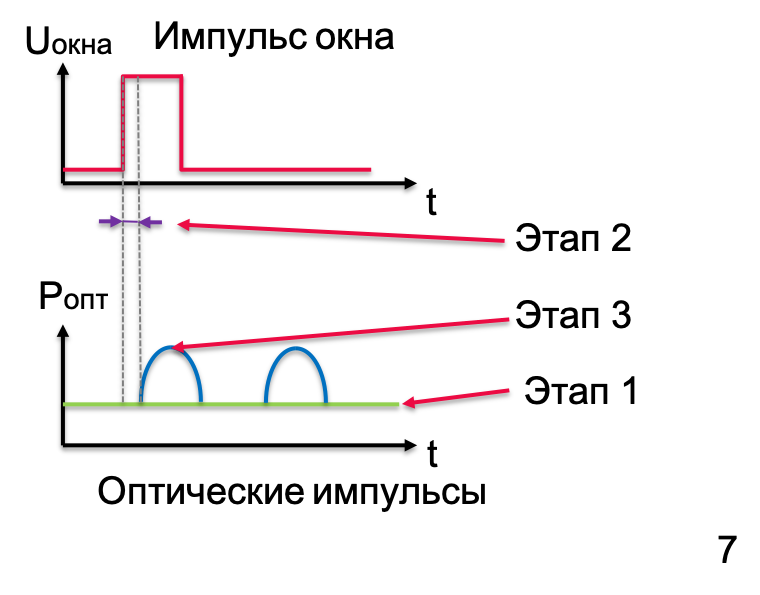
\includegraphics[scale=0.5]{Method_2.3.eps}
  \caption{Blinding methods}
  \label{fig:Method_2.3}
\end{figure}
%
 \begin{enumerate}
	\item Determining the constant optical power sufficient to switch the detector from the Geiger mode.
	\item Optical pulse adjustment for the SPD gate
	\item Dependence of the click probability on the photon energy in the trigger pulse value.
\end{enumerate}
%
As a result of the experimental study detector click probabilities were obtained (fig. \ref{fig:Probability_vs_Energy}). 

\begin{figure}[ht]
  \centering
  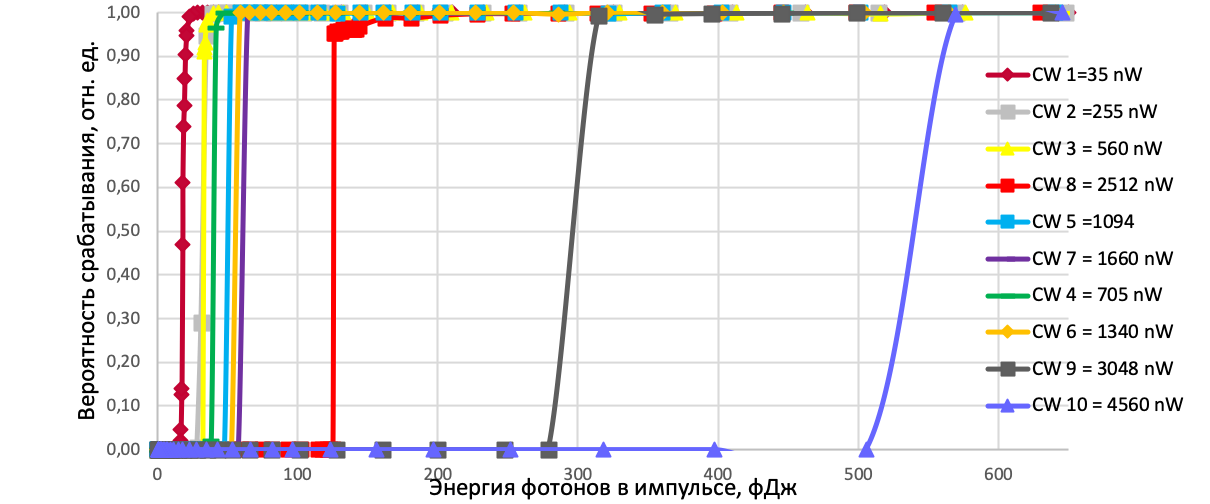
\includegraphics[scale=0.5]{Probability_vs_Energy.png}
  \caption{Detector click probability as a function of trigger pulse energy}
  \label{fig:Probability_vs_Energy}
\end{figure}


ТThus, it has been shown that the use of SPD based on APD in the Geiger mode (id210) with a gating frequency of 100~MHz requires the use of additional means of protection against attack with the switching from the Geiger mode using short optical pulses with an energy of at least 15.4~fJ and at a constant level of optical illumination with an average radiation power level of at least 35~nW. 

 \underline{\textbf{Третья глава}} посвящена исследованию предложенной автором работы атаки с навязыванием ключа на системы ККБЧ. Оценены границы применимости данной атаки с учетом характеристик и параметром оборудования в составе блока получателя. Для определения попыток злоумышленника провести описанную выше атаку предлагается измерять интенсивность центральной оптической моды. Центральная мода отражается узкополосным фильтром на основе брэгговской решетки. Для того, чтобы её можно было измерить в схеме устанавливается волоконно-оптический циркулятор. Все излучение, которое после фазовых модуляторов в приемном блоке поступает на первый порт циркулятора направляется во второй порт на оптический фильтр. Отраженная центральная мода направляется в третий порт циркулятора. Для того, чтобы измерять центральную, которая, как показано в разделе, должна быть порядка 700~нВт, предлагается использовать мониторный фотодиод. Так как. злоумышленника есть возможность подбирать интенсивность на центральной моде, то очевидным является то, что мониторный фотодиод, установленный на выходе с 3-го порта, можно также контролировать оптическими методами. Для того, чтобы избежать этого, предлагается использовать волоконно-оптическое зеркало, например широко доступное зеркало Фарадея, и пассивный оптический аттенюатор. Сам мониторный фотодиод предлагается устанавливать в 4-ом порту циркулятора. Таким образом, излучение с центральной модой поступает на 3-ий порт, проходит аттенюатор в прямом направлении, отражается от волоконного зеркала, проходит аттенюатор в обратном направлении и поступает на 4-й порт, где установлен мониторный фотодиод.         
 \begin{figure}[ht]
  \centering
  \includegraphics[scale=0.25]{scw-setup_Countermeasure.pdf}
  \caption{Принципиальная оптическая схема предлагаемой контрмеры против атаки с <<поддельными>> состояниями}
  \label{fig:countermeasure}
\end{figure}
 
 На рисунке \ref{fig:Watchdog_photodiode} представлены две зависимости: нижний предел -- величина оптической мощности, которая требуется для выведения детектора фотонов из режима Гейгера и является минимальной необходимой для проведения успешной атаки злоумышленником; верхняя граница - величина оптической мощности, которая получена исходя из параметров приёмного модуля системы квантовой коммуникации и ограничения сверху на величину оптической мощности контролирующих импульсов. Минимальный уровень в соотвествии с расчетом составляет 0.7~мкВт, а максимальный - величину порядка 300~мкВт (в рамках данного исследования), однако на деле ограничен пороговой величиной ЛФД внутри ДОФ, при достижении которой ток становится слишком большим и диод сгорает, выводя из строя всё устройство. Типичной величиной являются единицы и десятки милливатт. 


С учётом данной зависимости можно оценить величину ослабления в фиксированном аттенюаторе, которой будет достаточно для защиты мониторного фотодиода от засветки, и при этом не потребуются дополнительные меры по расширению динамического диапазона чувствительности к входной оптической мощности в сторону увеличения, так как при оптических мощностях ниже единиц нановатт погрешность измерений становится достаточно высокой.   

Исходя из этого, величины аттенюации в 10~дБ достаточно, так как отраженная центральная на выходе с 3-го порта циркулятора прохоит через ослабляющий элемент в первый раз, а затем после отражения от зеркала во второй раз. Результирующее ослабление на 20~дБ, или в 100 раз, снизит минимальный уровень мощности на центральной частоте, которого достаточно для выведения детектора из режима счета фотонов, до величины порядка 7~нВт, что удовлетворяет требованиям, описанным выше. Максимальный уровень (в рамках данного исследования) снизится при этом примерно до 3~мкВт. 

 \begin{figure}[ht]
  \centering
  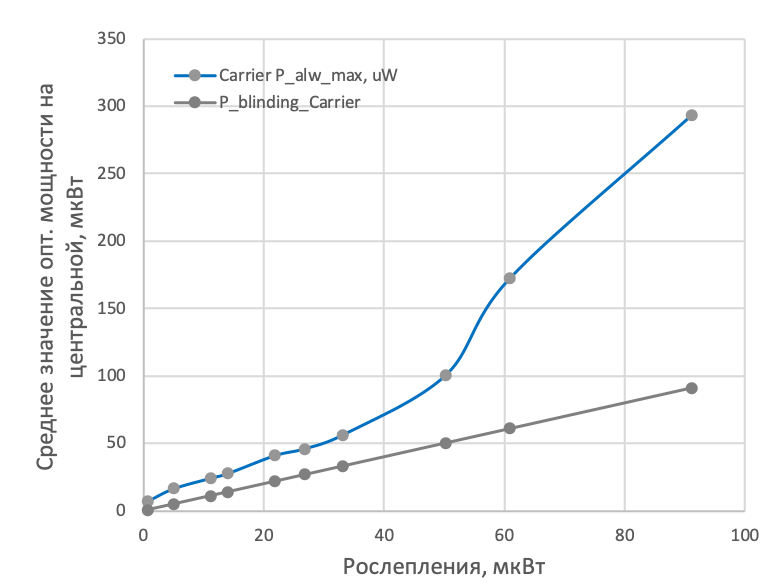
\includegraphics[scale=0.5]{images/Watchdog_photodiode.png}
  \caption{Динамика и границы оптической мощности на мониторном фотодиоде}
  \label{fig:Watchdog_photodiode}
\end{figure}


 В третьей главе показано, что измерение величины оптического излучения на несущей частоте, отраженного от оптического фильтра, при помощи мониторного фотодиода в приемном блоке системы квантовой коммуникации на боковых частотах в диапазоне от 7 нВт до 2,93 мкВт с применением дополнительных мер в виде пассивного оптического аттенюатора номиналом 10 дБ для его защиты позволяет противостоять атаке с выведением детектора одиночных фотонов из режима Гейгера и навязыванием ключа нелегитимным пользователем. 

% Можно сослаться на свои работы в автореферате. Для этого в файле
% \verb!Synopsis/setup.tex! необходимо присвоить положительное значение
% счётчику \verb!\setcounter{usefootcite}{1}!. В таком случае ссылки на
% работы других авторов будут подстрочными.
% \ifnumgreater{\value{usefootcite}}{0}{
% Изложенные в третьей главе результаты опубликованы в~\cite{vakbib1, vakbib2}.
% }{}
% Использование подстрочных ссылок внутри таблиц может вызывать проблемы.

 В \underline{\textbf{четвертой главе}} приведено описание когерентных состояний, которые нашли широкое применение в системах квантовой коммуникации, ввиду того, что в качестве источника излучения используются когерентные лазеры. 
 
 Отличительно особенностью систем квантовой коммуникации на боковых частотах модулированного излучения является генерация многомодовых когерентных состояний на разных оптических модах, зависящих от частоты модулирующего сигнала, как показано на рисунке \ref{fig:multimodes}. 

 \begin{figure}[ht]
  \centering
  \includegraphics[scale=0.4]{Modes_rus.pdf}
  \caption{Принципиальная схема генерации боковых частот}
  \label{fig:multimodes}
\end{figure}


Определим приготовленные состояния. Входное (немодулированное) состояние на стороне модулятора отправителя (Алиса) и получателя (Боб) (далее именуемые, как $A$ or $B$) определяется, как $|\sqrt{\mu_0}\rangle_0\otimes|\mathrm{vac}\rangle_{SB}$, где $|\mathrm{vac}\rangle_{SB}$ это вакуумное состояние на боковых и $|\sqrt{\mu_0}\rangle_0$ это когерентное состояние несущей частоты с амплитудой, определенной средним числом фотонов $\mu_0$ в окне пропускания. формируемая когерентным монохроматическим излучением с оптической частотой $\omega$. Фаза несущей волны принимается как опорная и все остальные фазы считаются по отношению к ней. Электро-оптический фазовый модулятор (с частотой колебаний микроволнового поля $\Omega$ и её фазой $\varphi_A$ или $\varphi_B$) перераспределяет энергию между взаимодействующими модами (поле на выходе модулятора приобретает боковые частоты $\omega_k=\omega+k\Omega$, ограничим рассматриваемый нами случай $2S$ боковыми частотами и пусть целое число $k$ мод ограничено пределами $-S\le k\le S$), так, что состояние поля на выходе модулятора - это многомодовое когерентное состояние: 
%
\begin{equation}\label{phi}
|\psi_0(\varphi_j)\rangle = \bigotimes_{k=-S}^S|{\alpha_k(\varphi_j)}\rangle_k,
\end{equation}
%
где $j$ это и $A$, и $B$ (определяющее Алису или Боба), а амплитуды имеют следующий вид: 
%
\begin{equation}\label{alpha}
\alpha_k(\varphi_j)=\sqrt{\mu_0}d^S_{0k}(\beta)e^{i\varphi_jk},
\end{equation}
%
и $d^S_{nk}(\beta)$ это d-функция Вигнера, взятая из квантовой теории углового момента %\cite{varshalovich1988quantum}
, $\beta$ определяется индексом модуляции $m$, который без учета дисперсии в среде модулятора можно выразить: 
%
\begin{equation}\label{betam}
\cos{({\beta})}=1-\frac{1}{2}{\left(\frac{m}{S+0.5}\right)^2},
\end{equation}
где $S$ количество взаимодействующий мод, принимаемое очень большим.

После подстройки относительной фазы оптических сигналов в двух плечах, наблюдается интерференция этих состояний на втором светоделителе ($BS2$). Описание состояний на выходах светоделителя дано в уравнении~\ref{states}. Далее предполагается, что относительная фазовая отстройка оптических импульсов равна $\phi_0\approx0$. Если разность фаз между радиочастотными модулирующими сигналами Алисы и Боба равна нулю ($\Delta\varphi=0$) весь спектр идет в одно выходное плечо светоделителя $BS2$, в ином случае, четные моды спектра, включая центральную, идут в то же плечо, а нечетные идут во второе плечо. В случае $\Delta\varphi=0$, требуется спектральное разделение центральной частоты и боковых в приёмном блоке, так как кодирование квантовых состояний происходит на боковых частотах. Следует учитывать, что при использовании малого среднего числа фотонов в импульсе, значительный вклад в многомодовых состояниях вносят только первая пара боковых частот. Случай, при котором $\Delta\varphi=\pi$, является нетривиальным. Многомодовое состояние разделяется на $BS2$ и центральная мода (и все четные) идут в первое плечо, а все нечетные (первые боковые частоты вносят наибольший вклад в результирующий сигнал) идут во второе плечо, как показано на рисунке \ref{fig:Interference_result}. Таким образом, можно отказаться от спектрального разделения при помощи оптического фильтра в одном из выходных плечей приёмного узла. Показателем хорошей подстройки по фазе оптических импульсов является постоянный высокий уровень на центральной частоте в первом плече (на $D2$).  


\begin{figure}[ht]
 \centering
  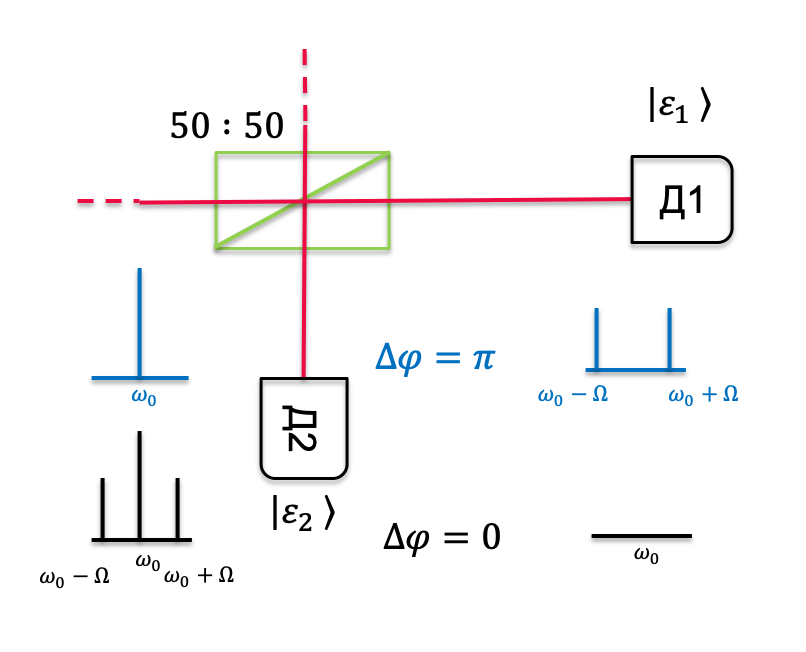
\includegraphics[scale=0.5]{Interference_result.png}
  \caption{Принципиальная схема наблюдения результата интерференции когерентных состояний}
  \label{fig:Interference_result}
\end{figure}

 
В четвертой главе показано, что метод квантовой коммуникации на боковых частотах позволяет реализовывать протокол, устойчивый к контролю нелегитимным пользователем измерительного оборудования. 

Основываясь на полученных результатах можно сформулировать протокол для системы квантовой коммуникации, использующей многомодовые когерентные состояния, с недоверенным измерительным узлом (рис. \ref{fig:Protocol}). Для простоты приведем пример с использованием только двух фазовых состояний по аналогии с протоколом B92. Алиса случайным образом выбирает одно фазовое состояние из двух возможных <<$0$>> или <<$\pi$>>. Боб независимо от Алисы тоже случайным образом выбирает одно из двух фазовых состояний. В результате интерференции многомодовых когерентных состояний можно наблюдать 4 различных варианта, в зависимости от разности фаз, выбранных Алисой и Бобом.  При этом на недоверенном узле регистрации будет происходить спектральное разделение, так что на $D1$ и $D2$ будут поступать боковые частоты. Злоумышленник при этом имеет полный доступ к недоверенному измерительному узлу и может фиксировать себе оглашенный результат срабатываний одного из детекторов. Положим, что нас интересует только случай, при котором разность фаз между $A$ и $B$ равна $\pi$. Преимущество этого случая в том, что за счет спектрального разделения в результате интерференции в плечо с детектором $D1$ всегда будут идти только боковые и никогда не будет идти центральная мода, а значит можно исключить из оптической схемы этого плеча оптический фильтр, согласование которого с фильтром в другом плече -- достаточно трудная инженерная задача. Таким образом, при просеивании остаются только те биты, которые соответствуют отсчетам на $D1$, при этом для корреляции между битами Алисы и битами Боба последний должен сделать смену бита на противоположный (так называемый <<bitflip>>).  

\begin{figure}[ht]
 \centering
  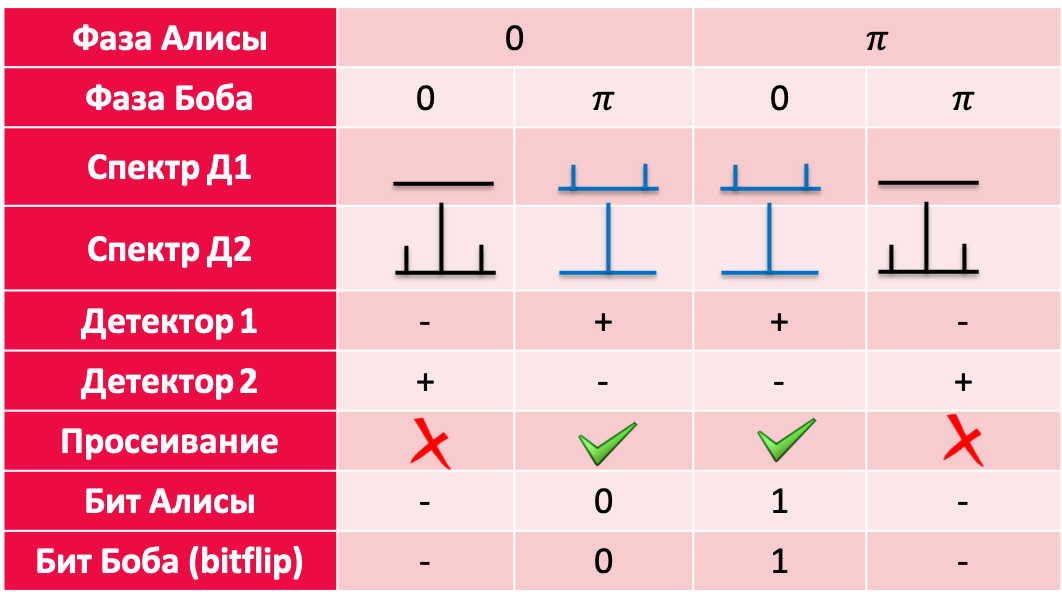
\includegraphics[scale=0.5]{Protocol.png}
  \caption{Протокол}
  \label{fig:Protocol}
\end{figure}
 
  В \underline{\textbf{пятой главе}} показано, что в результате интерференции квантового фазомодулированного сигнала на боковых частотах на симметричном светоделителе в схеме квантовой рассылки ключа с узлом регистрации, независящим от легитимного пользователя, происходит спектральное разделение квантового сигнала и сигнала на центральной длине волны с их независимой регистрацией в разных плечах светоделителя. 
  
  Для проверки концепции была собрана оптическая схема, представленная на рисунке \ref{fig:RF_sin}. Для простоты использовался только один источник излучения, сигнал на выходе которого делился светоделителем 50:50 $BS1$. Такой подход позволяет имитировать случай, когда у Алисы и Боба хорошо скоррелированные источники излучения. В данном эксперименте применялся лазер с распределенной обратной связью Л1 (TTX1994 Neophotonics), отличительными особенностями которого являются очень узкая ширина спектральной линии порядка 100~кГц и широкий диапазон перестройки длин волн (от 1530~нм до 1565,5~нм) с высокой степенью точности (20~пм). Выходная мощность при этом составляла 10~мВт. Однако, это значение зависит от глубины динамического диапазона перестраиваемого оптического аттенюатора ПОА и суммарных потерь, вносимых элементами Алисы или Боба, так как результирующая мощность сигнала на боковых частотах должна не превышать величину 2,56~пВт, соответствующую среднему числу фотонов в импульсе 0,2 при частоте смены состояний 100~Мгц.   

Из-за чувствительности резонатора внутри лазера с распределенной обратной связью к обратному относительно выходного оптическому излучению, то есть переотражениям и рассеиванию сигналов, в оптической схеме применяется волоконный изолятор И на основе эффекта Фарадея с величиной изоляции порядка 50~дБ. Для перевода системы в однофотонный режим применяется ПОА с достаточной малым шагом перестройки 0,05 дБ и большим динамическим диапазоном величиной 60~дБ.  

  

  \begin{figure}[ht]
  \centering
  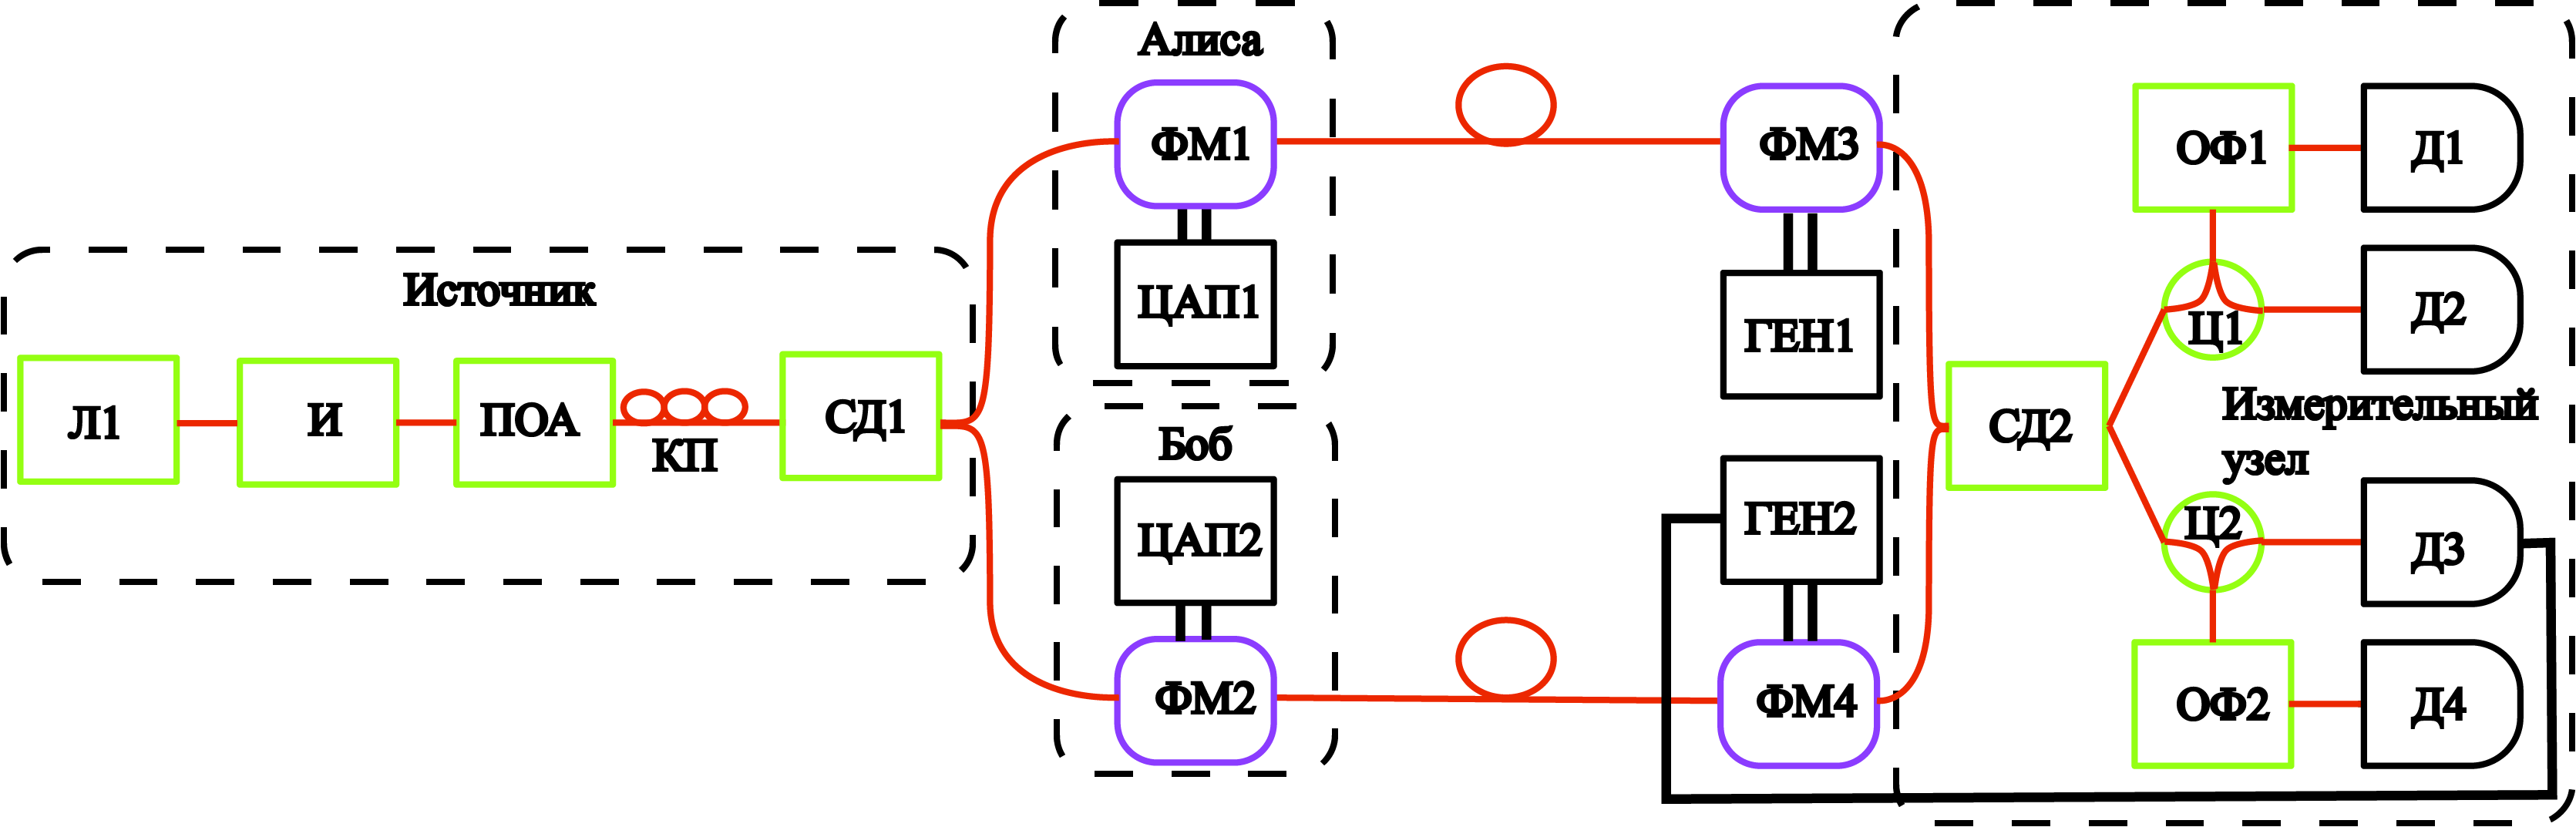
\includegraphics[scale=0.4]{Scheme_colored_rus.png}
  \caption{Принципиальная схема экспериментального стенда}
  \label{fig:RF_sin}
\end{figure}

  
 
  
На выходе из источника сигнал проходил по двум плечам формируемого таким образом интерферометра через светоделитель, благодаря чему имитировалось, что Алиса и Боб - это раздельные узлы, в которых информация кодировалась с помощью фазовых модуляторов. Выходы первого светоделителя подключались ко входам двух независимых 10~ГГц электро-оптических модуляторов на основе $LiNbO_3$ (со встроенным поляризатором) $PM1$ and $PM2$. Поляризаторы снижали чувствительность модуляторов к поляризации входного излучения, для чего использовался контроллер поляризации КП, и таким образом, повышалась видность картины интерференции. Электрические входы $PM1$ и $PM2$ подключались к выходам с цифро-аналоговых преобразователей ЦАП с модулирующим радиочастотным синусоидальным сигналом (с частотой 4,8~ГГц). Амплитуды управляющих сигналов подбирались таким образом, чтобы мощность сигнала на боковых частотах была равно у Алисы и у Боба

Индекс модуляции, который показывает долю энергии на боковых частотах по отношению к центральной в результате модуляции должен быть 5~\%. В таком случае наблюдается оптимальное соотношение сигнала на боковых частотах к шуму проходящей через оптический фильтр центральной частоты.  Так что средняя величина оптической мощности была равна 2.56~пВт, что соответствует $\mu=0.2$.  


В данном исследовании  использовались только два кодирующих фазовых состояния на Алисе и Бобе ($\varphi_{A,B}\in\{0,\pi\}$. Разница фаз ($\Delta\varphi$) между Алисой и Бобом формировалась с помощью изменения IQ-таблиц ЦАП при помощь ПЛИС и ПО сосбтвенной разработки. В случае измерения зависимости количества срабатываний детекторов от разности фаз ($\Delta\varphi$) фаза сдвигалась последовательно с шагом $\varphi_{step}\ = 10^{\circ}$. Наблюдаемые состояния на выходах $PM1$ и $PM2$ могут быть описаны в соотвествии с уравнением~\ref{phi}.

После того, как состояния приготовлены, мы посылаем их в квантовый канал. Для компенсации оптической разности хода в двух плечах интерферометра, а так же для точной подстройки оптических фаз сигналов использовались $PM3$ и $PM4$. Эта подстройка осуществлялась при помощи изменения постоянного напряжения, подаваемого на модуляторы и формируемого двумя независимыми электрическими выходами генератора сигналов $GEN1$ и $GEN2$. Выходы втрой пары фазовых модуляторов подключались к паре входных портов светоделителя $BS2$ 2x2 с коэффициентом деления 50:50.

Измерения проводились в два этапа: первый этап в классическом свете, второй этап - в режиме счета фотонов на сверхпроводниковом детекторе одиночных фотонов (Сконтел), у которого встроены два независимых приёмника $D1$, $D4$. Квантовая эффективность обоих была равна 10~\%, а уровень темновых шумов не превышал 50~Гц для каждого. Измеренная величина суммарных шумов, включающих в себя темновые срабатывания и засветку от центральной частоты в силу ограниченной экстинкции оптического фильтра, составляла $\gamma_{темн}=1.5$ кГц.

Показаны зависимости интенсивности на боковых частотах в результате интерференции от разности фаз модулирующих сигналов в классическом режиме и в режиме счета фотонов. Оценены основные параметры, характеризующие систему квантовой коммуникации: квантовый коэффициент ошибок по битам (QBER) и среднее значение скорости формирования просеянного ключа $K$ (одинаковые биты между легитимными пользователями, но коррелирующие с возможным результатом у злоумышленника, что требует проведения процедуры усиления секретности) 



 \underline{\textbf{Заключение}} содержит список основных результатов, полученных в работе. 

% !_____!
  %% Согласно ГОСТ Р 7.0.11-2011:
%% 5.3.3 В заключении диссертации излагают итоги выполненного исследования, рекомендации, перспективы дальнейшей разработки темы.
%% 9.2.3 В заключении автореферата диссертации излагают итоги данного исследования, рекомендации и перспективы дальнейшей разработки темы.
\begin{enumerate}
  \item На основе экспериментального анализа детектора, работающего в режиме Гейгера, показано, что требуются дополнительные средства защиты от атаки с выведением из режима Гейгера при помощи коротких оптических импульсов с энергией не менее 15,4 фДж и при постоянном уровне оптической засветки средним уровнем мощности излучения не менее 35 нВт. 
  \item Численные исследования показали, что измерение величины оптического излучения на несущей частоте, отраженного от оптического фильтра, при помощи мониторного фотодиода в приемном блоке системы квантовой коммуникации на боковых частотах в диапазоне от 7 нВт до 2,93 мкВт с применением дополнительных мер в виде пассивного оптического аттенюатора номиналом 10 дБ для его защиты позволяет противостоять атаке с выведением детектора одиночных фотонов из режима Гейгера и навязыванием ключа нелегитимным пользователем. 
  \item Метод квантовой коммуникации на боковых частотах позволяет реализовывать протокол, устойчивый к контролю нелегитимным пользователем измерительного оборудования.
  \item Для выполнения поставленных задач был создан экспериментальный стенд и в результате интерференции квантового фазомодулированного сигнала на боковых частотах на симметричном светоделителе в схеме квантовой рассылки ключа с узлом регистрации, независящим от легитимного пользователя, наблюдается спектральное разделение квантового сигнала и сигнала на центральной длине волны с их независимой регистрацией в разных плечах светоделителя. 
\end{enumerate}

%	\newcommand{\publications}{\underline{\textbf{\publicationsTXT}}}

{The main results of the dissertation are listed in following publications, included in Scopus and Web of Science:}
\begin{enumerate}\addtolength{\itemsep}{-0.5\baselineskip}
\renewcommand{\labelenumi}{[\theenumi]}
\item Vladimir Chistiakov, Anqi Huang, Vladimir Egorov, and Vadim Makarov, Controlling single-photon detector ID210 with bright light, Opt. Express 27, 32253-32262 (2019)
\\
\item Чистяков В.В., Гайдаш А.А., Козубов А.В., Глейм А.В. Исследование интерференции слабых когерентных многомодовых состояний для задач квантовой коммуникации с недоверенным приемным узлом // Научно-технический вестник информационных технологий, механики и оптики. 2019. Т. 19. № 6. doi: 10.17586/2226-1494-2019-19-6
\\
\item    Gleim A.V., Egorov V.I., Nazarov Y.V., Smirnov S.V., Chistyakov V.V., Bannik O.I., Anisimov A.A., Kynev S.M., Ivanova A.E., Collins R.J., Kozlov S.A., Buller G. Secure polarization-independent subcarrier quantum key distribution in optical fiber channel using BB84 protocol with a strong reference//Optics express, IET - 2016, Vol. 24, No. 3, pp. 2619-2633
\\
\item  Глейм А.В., Егоров В.И., Чистяков В.В., Смирнов С.В., Банник О.И., Булдаков Н.В., Гайдаш А.А., Козубов А.В., Васильев А.Б., Кынев С.М., Хоружников С.Э., Козлов С.А., Васильев В.Н. Квантовая коммуникация на боковых частотах со скоростью 1 Мбит/с в городской сети // Оптический журнал -2017. - Т. 84. - № 6. - С. 3-9
\\
\item  Chistyakov V.V., Kynev S.M, Smirnov S.V., Nazarov Y.V., Gleim A.V. Achieving high visibility in subcarrier wave quantum key distribution system // Journal of Physics: Conference Series, IET - 2016, Vol. 735, No. 1, pp. 012085
\\
\item V. V. Chistyakov, A. V. Gleim, V. I. Egorov, Yu. V. Nazarov. Implementation of multiplexing in a subcarrier-wave quantum cryptography system // Journal of Physics: Conference Series - 2014  vol. 541,  pp. 012078
\\
\item   Kynev S.M., Chistyakov V.V., Smirnov S.V., Volkova K.P., Egorov V.I., Gleim A.V. Free-space subcarrier wave quantum communication // Journal of Physics: Conference Series - 2017, Vol. 917, No. 5, pp. 052003
\\

\item    Gleim A.V., Nazarov Y.V., Egorov V.I., Smirnov S.V., Bannik O.I., Chistyakov V.V., Kynev S.M., Anisimov A.A., Kozlov S.A., Vasil'ev V.N. Subcarrier Wave Quantum Key Distribution in Telecommunication Network with Bitrate 800 kbit/s//EPJ Web of Conferences, IET - 2015, Vol. 103, pp. 10005
\\
\item    Gleim A.V., Egorov V.I., Nazarov Y.V., Smirnov S.V., Chistyakov V.V., Bannik O.I., Anisimov A.A., Kynev S.M., Collins R.J., Kozlov S.A., Buller G.S. Polarization insensitive 100 MHz clock subcarrier quantum key distribution over a 45 dB loss optical fiber channel // Conference on Lasers and Electro-Optics, CLEO 2015, IET - 2015, pp. 7182997
\\
\item Gaidash A.A., Kozubov A.V., Chistyakov V.V., Miroshnichenko G.P., Egorov V.I., Gleim A.V. Security conditions for sub-carrier wave quantum key distribution protocol in errorless channel // Journal of Physics: Conference Series - 2017, Vol. 917, No. 6, pp. 062014
\\
%\item  Gleim A.V., Chistyakov V.V., Bannik O.I., Egorov V.I., Buldakov N.V., Vasilev A.B., Gaidash A.A., Kozubov A.V., Smirnov S.V., Kynev S.M., Khoruzhnikov S.E., Kozlov S.A., Vasil'ev V.N. Sideband quantum communication at 1 Mbit/s on a metropolitan area network // Journal of Optical Technology - 2017, Vol. 84, No. 6, pp. 362-36
\\

\end{enumerate}
\noindent{Other publications:}
\begin{enumerate}\addtolength{\itemsep}{-0.5\baselineskip}
\renewcommand{\labelenumi}{[\theenumi]}
\setcounter{enumi}{9}
\item   Чистяков В.В., Кынев С.М., Смирнов С.В., Назаров Ю.В., Глейм А.В. Обеспечение высокой видности в системе квантовой криптографии на боковых частотах // Сборник трудов IX международной конференции молодых ученых и специалистов «Оптика – 2015», с. 658-660
\\
\item Глейм А.В., Назаров Ю.В., Егоров В.И., Чистяков В.В, Смирнов С.В., Банник О.И., Кынев С.М., Иванова А.Е., Дубровская В.Д., Тарасов М.Г., Булдаков Н.В., Кузьмина Т.Б., Чивилихин С.А., Анисимов А.А., Рощупкин С.В., Рогачёв К.С., Хоружников С.Э., Козлов С.А., Васильев В.Н. Создание квантовой сети университета ИТМО //Сборник трудов VIII международной конференции «Фундаментальные проблемы оптики – 2014». Санкт-Петербург, 20-24 октября ,2014, С.3-4,  541 с. 
\\
\item А.В. Глейм, В.И.Егоров, А.А. Анисимов, Ю.В. Назаров, С.М. Кынев, А.В. Рупасов, В.В. Чистяков, А.А.Гайдаш, М.А. Смирнов, С.А. Чивилихин, С.А. Козлов Квантовая рассылка криптографического ключа по оптическому волокну телекоммуникационного стандарта на расстояние 200 км со скоростью 0.18 кбит/с // Cборник трудов III Всероссийская конференция по фотонике и информационной оптике Москва, НИЯУ МИФИ, 2014 с. 17-19
\\


\end{enumerate}


%При использовании пакета \verb!biblatex! список публикаций автора по теме
%диссертации формируется в разделе <<\publications>>\ файла
%\verb!../common/characteristic.tex!  при помощи команды \verb!\nocite!

\ifdefmacro{\microtypesetup}{\microtypesetup{protrusion=false}}{} % не рекомендуется применять пакет микротипографики к автоматически генерируемому списку литературы
\ifnumequal{\value{bibliosel}}{0}{% Встроенная реализация с загрузкой файла через движок bibtex8
  \renewcommand{\bibname}{\large \authorbibtitle}
  \nocite{*}
  \insertbiblioauthor           % Подключаем Bib-базы
  %\insertbiblioother   % !!! bibtex не умеет работать с несколькими библиографиями !!!
}{% Реализация пакетом biblatex через движок biber
  \ifnumgreater{\value{usefootcite}}{0}{
%  \nocite{*} % Невидимая цитата всех работ, позволит вывести все работы автора
  \insertbiblioauthorcited      % Вывод процитированных в автореферате работ автора
  }{
  \insertbiblioauthor           % Вывод всех работ автора
%  \insertbiblioauthorgrouped    % Вывод всех работ автора, сгруппированных по источникам
%  \insertbiblioauthorimportant  % Вывод наиболее значимых работ автора (определяется в файле characteristic во второй section)
  \insertbiblioother            % Вывод списка литературы, на которую ссылались в тексте автореферата
  }
}
\ifdefmacro{\microtypesetup}{\microtypesetup{protrusion=true}}{}
